\chapter{Methodology}

This chapter outlines the methodologies employed in our study. In Section I we begin with a discussion of the datasets used. In Section II, we explore the application and customization of SimCLR and t-SimCNE. In Section III we describe our hard negative sampling approach.
Section IV introduces the AUC-CL framework we used to incorporate the Area under the ROC curve metric.

\section{Datasets}
\subsection{CIFAR-10}
The CIFAR-10 dataset \cite{cifar10} comprises 60,000 images in 32x32 resolution, each in full color, and is distributed evenly across 10 classes. This dataset is commonly used for benchmarking image recognition algorithms, providing a diverse range of object classes to test the robustness and generalizability of models.


\subsection{MedMNIST}
Medmnist \cite{medmnist} is a standardized collection of medical image datasets for deep learning benchmarks. It includes different medical imaging data, such as dermatological, radiological, and hematological images. We used Dermamnist and Bloodmnist datasets.

Dermamnist dataset contains 10,015 dermatological images, each resized to 28x28 pixels in grayscale. These images are categorized into seven classes. This subset of Medmnist is designed for the task of skin disease classification.

Bloodmnist dataset includes 17,092 microscopic images of blood cells, standardized to 28x28 pixel grayscale images. These images are categorized into eight types. Bloodmnist facilitates the training of models for the classification of blood cells, aiding in the diagnosis of hematological diseases.

\subsection{Leukemia}
The Leukemia dataset \cite{leukemia} consists of microscopic images of white blood cells sourced from patients, including those diagnosed with leukemia. The original resolution is 224 x 224, so we downscaled these images to 28 x 28 to align with the MedMNIST standards.


\section{SimCLR algorithm}
SimCLR (Simple Contrastive Learning of Representations) is a self-supervised learning framework designed to learn visual representations without requiring labeled data. The core idea of SimCLR is to maximize agreement between differently augmented views of the same image via a contrastive loss. This method operates in several steps:

\subsection{Data Augmentation}
Each image in the dataset is transformed twice using random data augmentation techniques such as cropping, resizing, color distortion, and Gaussian blurring to generate two correlated views, denoted as positive pairs. 

\subsection{Feature Extraction}
Both augmented images are then fed into a shared convolutional neural network to extract features.

\subsection{Projection Head}
The representations are then passed through a projection head, which is a small feed-forward neural network, to obtain the final representations used in the contrastive loss calculation.

\subsection{Contrastive Loss}
SimCLR utilizes the contrastive loss function known as normalized temperature-scaled cross-entropy loss (NT-Xent). The loss function for a positive pair of examples $(i, j)$ is given by:

\begin{equation}
\ell(i, j) = -\log \frac{\exp(\text{sim}(z_i, z_j) / \tau)}{\sum_{k=1}^{2N} \mathbf{1}_{[k \neq i]} \exp(\text{sim}(z_i, z_k) / \tau)}
\end{equation}

where $\text{sim}(u, v) = \frac{u^\top v}{\|u\| \|v\|}$ denotes the cosine similarity between $u$ and $v$, $\tau$ is a temperature scaling parameter, and $N$ is the batch size. The indicator function $\mathbf{1}_{[k \neq i]}$ is 1 iff $k \neq i$ and ensures that a sample does not form a negative pair with itself.

This loss function encourages representations of positive pairs to be closer to each other while pushing representations of negative pairs (different images) apart in the embedding space.

\section{Extension of SimCLR with t-SimCNE}
\subsection{Overview}
We used t-SimCNE (t-distributed Simultaneous Contrastive Neighbor Embedding) to extend the SimCLR framework by optimizing direct mapping from the high-dimensional pixel space to a two-dimensional embedding space. This method is designed to produce meaningful and interpretable visualizations of image datasets by preserving semantic relationships within the data.

t-SimCNE modifies the typical contrastive learning approach by using a two-dimensional output directly during the training phase rather than using the high-dimensional outputs typical of models like SimCLR. This approach allows for immediate data visualization without additional dimensionality reduction steps.

\begin{figure}[hbt]
\centering
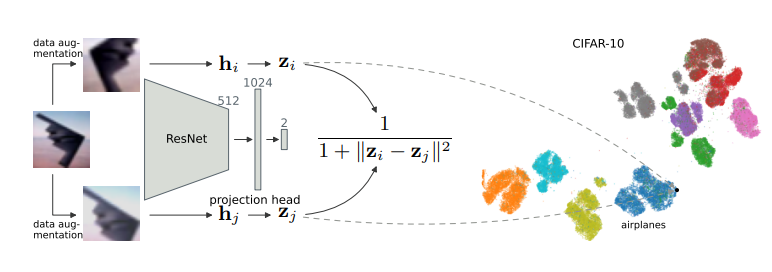
\includegraphics[width=\textwidth]{figs/tsimcne_architecture.png}
\caption{
t-SimCNE algorithm \cite{tsimcne}.
}
\label{fig:secex}
\end{figure}

\subsection{t-SimCNE Loss Function}
The t-SimCNE modifies the contrastive loss function by incorporating the Cauchy kernel, which is particularly effective for handling the crowding problem at lower dimensions. The loss function is given by:

\begin{equation}
\mathcal{L}(i, j) = -\log \left(\frac{\frac{1}{1 + \|z_i - z_j\|^2}}{\sum_{k=1}^{2N} \mathbf{1}_{[k \neq i]} \frac{1}{1 + \|z_i - z_k\|^2}}\right)
\end{equation}

Here, $z_i$ and $z_j$ are the two-dimensional embeddings of two different augmented views of the same image, and $\|z_i - z_j\|^2$ represents the squared Euclidean distance between the embeddings $z_i$ and $z_j$. The temperature parameter traditionally used in the softmax function is implicit in the normalization by the Cauchy kernel, and $N$ is the batch size used during training.


\subsection{Training Strategy}
t-SimCNE involves several key stages in training:
\begin{itemize}
    \item Pre-training in a higher dimensional space (typically 128D) to stabilize the learning of useful features.
    \item Fine-tuning the network to produce 2D outputs for direct visualization.
    \item An additional fine-tuning phase over the entire network to refine the embeddings and improve the visualization quality.
\end{itemize}


\section{Visualization Algorithms}
We tested different visualization algorithms to prove that t-SimCNE is the best one.

\subsection{Standalone t-SNE}

t-SNE is an algorithm used to visualize high-dimensional data in two or three dimensions. The algorithm works by converting similarities between data points to joint probabilities and minimizing the Kullback-Leibler divergence between the joint probabilities of the low-dimensional embedding and the high-dimensional data.

t-SNE starts by calculating probabilities in the high-dimensional space that are related to the similarity of data points:
\[
p_{j|i} = \frac{\exp(-\|x_i - x_j\|^2 / 2\sigma_i^2)}{\sum_{k \neq i} \exp(-\|x_i - x_k\|^2 / 2\sigma_i^2)}
\]
where \(p_{j|i}\) represents the probability that point \(x_j\) would be picked as a neighbor of point \(x_i\) under a Gaussian centered at \(x_i\) with variance \(\sigma_i^2\).

In the low-dimensional space, t-SNE defines a similar probability but using a Student-t distribution:
\[
q_{ij} = \frac{(1 + \|y_i - y_j\|^2)^{-1}}{\sum_{k \neq l} (1 + \|y_k - y_l\|^2)^{-1}}
\]
where \(y_i\) and \(y_j\) are the embeddings of points \(x_i\) and \(x_j\) in the low-dimensional space.

The goal of t-SNE is to minimize the difference between these probability distributions:
\[
C = \sum_i \sum_j p_{ij} \log\left(\frac{p_{ij}}{q_{ij}}\right)
\]

\subsection{t-SimCNE}
Unlike traditional dimensionality reduction methods, t-SimCNE integrates visualization directly into the learning process, turning complex image datasets into two-dimensional data without the need for postprocessing. This method addresses the limitations of t-SNE and UMAP by preserving both local and global structures within the data.

\subsection{t-SNE with SimCLR}
When combined with SimCLR, t-SNE is used to further process the 128-dimensional outputs generated by SimCLR. This method helps in identifying how similar or different the images are, simplifying the complexity of high-dimensional data for easier analysis. This integration provides a practical way to see and understand the natural groupings within a dataset.


\section{Hard Negative Sampling}
We integrated hard negative sampling into the t-SimCNE framework to refine the model's ability to differentiate between similar yet distinct image features effectively. This method addresses the challenge of selecting informative negatives without supervision.

\subsubsection{Importance}
Hard negative samples are those data points that are close to the anchor point in the embedding space but have different classes. By emphasizing these hard negatives, t-SimCNE can generate embeddings that more accurately reflect the underlying data structure and improve the separation between different classes in complex datasets.

\subsubsection{Mathematical Formulation}
The selection of hard negatives in the t-SimCNE is guided by a sampling distribution, which prefers negatives whose representations are very similar to the anchor, providing a stronger gradient during training. This can be mathematically represented as:

\begin{equation}
q_{\beta}(x^-) \propto \exp(\beta \cdot f(x)^T f(x^-)) \cdot p(x^-)
\end{equation}

where $f(x)$ and $f(x^-)$ are the features of the anchor and negative samples, respectively, $\beta$ is a parameter controlling the "hardness" of the negatives, and $p(x^-)$ is the probability distribution of the negatives.

\subsubsection{Implementation in t-SimCNE}
To incorporate hard negative sampling into t-SimCNE, we adjust and weigh the selected hard negatives more heavily during the contrastive loss computation. This adjustment helps focus on critical features for distinguishing between similar yet categorically different images.

\section{AUC-CL Framework}
The AUC-Contrastive Learning (AUC-CL) framework further enhances our contrastive learning approach by integrating the Area under the receiver operating characteristic (ROC) curve (AUC) maximization into the learning objective. This method addresses the limitations of contrastive learning related to batch size sensitivity and optimization biases.

\subsection{Motivation and Definition}
In contrastive learning, the choice of batch size can significantly impact performance due to the biased estimation of gradients from small sample sizes. AUC-CL proposes to resolve this using the AUC metric, which evaluates the probability that a randomly chosen positive instance is ranked higher than a randomly chosen negative instance. The goal is to maximize this probability, ensuring that positive pairs have higher similarity scores than negative pairs.

\subsection{AUC Maximization}
The Area Under the Receiver Operating Characteristic Curve (AUC-ROC) is a measure of the ability of a classifier to distinguish between classes. For a binary classifier \( h_w \) parameterized by \( w \) with labeled samples \( \{x, x'\} \) where \( y = 1 \) and \( y' = -1 \) represent positive and negative classes respectively, the AUC is defined as:

\[
AUC(w) = P(h_w(x) \geq h_w(x') \mid y = 1, y' = -1)
\]

This equation states that the AUC is the probability that a randomly chosen positive example is scored higher by the classifier than a randomly chosen negative example.

The direct computation of AUC involves considering all possible pairs of positive and negative samples. For a dataset with \( N \) samples, if the numbers of positive and negative samples are approximately equal, this leads to \( O(N^2) \) complexity. This is because each positive sample is compared against each negative sample to compute the AUC, which becomes computationally intensive for large datasets.

To address the computational challenge, we reformulate it using a square loss function:

\[
L(w) = E\left[(1 - h_w(x) + h_w(x'))^2 \mid y = 1, y' = -1\right]
\]

This loss function simplifies the optimization problem by transforming the original probability comparison into a squared error term, which is easier to handle computationally. The expectation \( E \) averages over all positive-negative pairs, but the squared term allows the gradient of the loss with respect to the parameters \( w \) to be computed more efficiently. 

Minimizing the previous equation, we get the final loss function.

\subsection{AUC-CL Loss Function}
The AUC-CL framework is as follows:
\[
L'_s(w, b; x_i, A, A', B_i) = A_1 + A_2 + A_3
\]
where
- \(A_1\): Positive pair term, penalizing the distance between embeddings of the same image under different augmentations.
  \[
  A_1 = \left[ (\text{sim}(i, i+) - a)^2 \right] \text{ where } y_{ii+} = 1
  \]

- \(A_2\): Negative pair term, penalizing the closeness between embeddings of different images.
  \[
  A_2 = \sum_{j \in B_i} \left[ (\text{sim}(i, j) - b)^2 \right] \text{ where } y_{ij-} = 1
  \]

- \(A_3\): Regularization term to balance the contribution of positive and negative pairs.
  \[
  A_3 = \left\{ 2\alpha \left[ 1 - \text{sim}(i, i+) + \sum_{j \in B_i} \text{sim}(i, j) \right] - \alpha^2 \right\}
  \]

The variables are:
- \(w, b\): Parameters to optimize.
- \(x_i\): Training sample.
- \(A, A'\): Augmentation functions.
- \(B_i\): Batch subset excluding \(x_i\).
- \(\text{sim}(i, j)\): Similarity measure, typically cosine similarity.
- \(a, b\): Baseline similarities for positive and negative pairs.
- \(\alpha\): Scaling factor for the regularization term.


\begin{figure}[hbt]
\centering
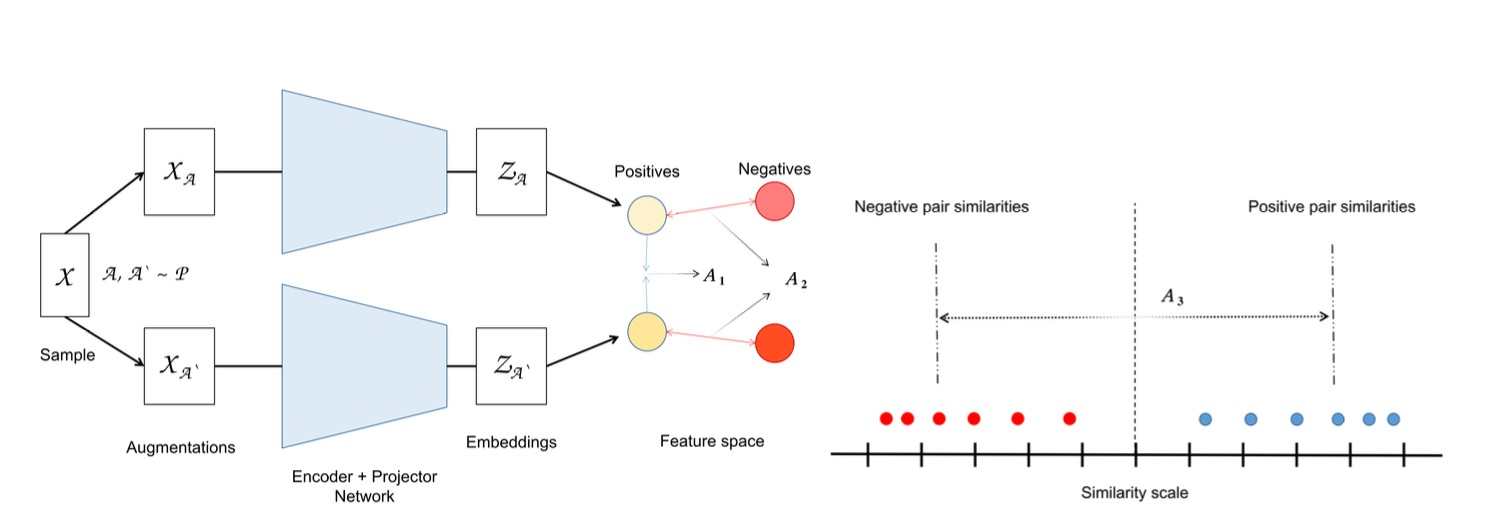
\includegraphics[width=\textwidth]{figs/auc-cl.png}
\caption{
AUC-CL schema \cite{sharma2023auc}.
}
\label{fig:secex}
\end{figure}

\subsection{Optimization and Robustness}
The integration of the AUC into the contrastive learning framework helps stabilize the training under conditions of limited computational resources or smaller batch sizes. This stability is due to the unbiased nature of the gradient updates provided by the AUC component, which does not suffer from the large variance typically seen with small batches in traditional contrastive learning setups.
